\documentclass[12pt,a4paper]{article}		% Necessary line
\usepackage{graphicx}		% Necessary line
\usepackage{mathtools}
\usepackage{breqn}
\usepackage{float}
\usepackage{caption}
\usepackage{subcaption}
\usepackage{hyperref}




\usepackage[margin=.6in,footskip=0.25in]{geometry}


\title{\textbf { Generator level study of Z decay to muon pair events in pp collisions at $\sqrt{s}=13$ TeV}}
 
 
\author{Shubham P. Raghuvanshi\\Supervisor : Prof.Kajari Majumdar\\Department of High Energy Physics, TIFR, Mumbai.}

% Start the document
\begin{document}		% Necessary line: starts the document
\maketitle


In this work we present a generator level study of the characteristics of Drell-Yan process $Z \to \mu^+\mu^-$ using Monte-Carlo simulations of pp collision events at center-of-mass energy $\sqrt{s}=13$ TeV.


$Keywords :$ Z boson, Drell-Yan, Monte-Carlo.  

\newpage

\tableofcontents
\newpage
\section{Introduction}

All the particles in the standard model have weak interaction which is mediated by $W^\pm $ and Z particles. Due to extremely short lifetime Z boson cannot be detected directly in the experiment; therefore it's production is inferred only from its decay products. The signal has to be identified using the characteristics of the decay products against all other processes with same or similar final state. Though Z boson was discovered in 1983 through Drell-Yan process $q\bar{q} \to Z/\gamma* \to \ell^+\ell^-$, it has always been one of the benchmark  process at hadron colliders, even today due to its relatively clean final state and precise prediction of its rate from theory which helps to test standard model at higher energies. Furthermore, at the LHC, many aspects of the experiments are studied via Drell--Yan process. 
%The measured values of mass and width and production cross sections were in perfect agreement with the predictions of electroweak theory. The mass and decay width of Z boson are measured to be about 91.2 GeV and 2.5 GeV respectively. 
In this report we present a generator level study of the Z boson decay to di-muon and the corresponding event characteristics in pp collisions at centre-of-mass energy $\sqrt{s}=13$ TeV.


\section{The CMS detector}


Situated in the Franco-Swiss region of Geneva, \textbf{CMS(Compton muon solenoid)} is one  of two large general-purpose detector along with \textbf{ATLAS (A Toroidal
LHC Apparatus)} at the Large Hadron Collider (LHC) of CERN. The CMS detetcor is 21.6 meters in length, 15 meters in diameter and weighs about 14000 tons. Research goals in CMS include the study of and beyond standard model physics, search and study of Higgs particle, dark matter, extra dimensions. It was one of the two experiments which proved the existence of the Higgs particle in July 2012. Drell-Yan process was used for various calibration towards discovery of Higgs boson.  Figure~\ref{fig:CMS} displays a transverse slice of the cartoon of CMS detector

\begin{figure}[h]
	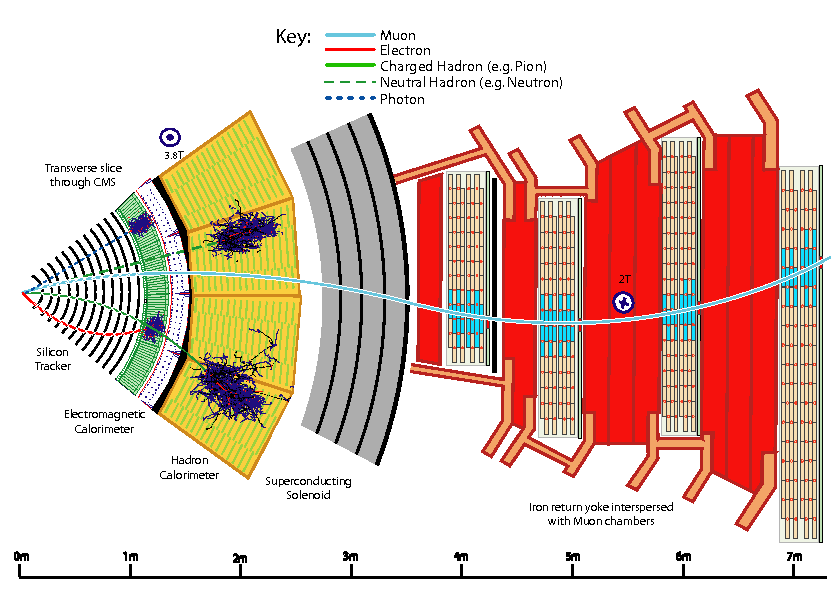
\includegraphics[scale=0.6]{cms.png} 
	\caption{Cross setion of the CMS detector normal to the beam axis}
   \label{fig:CMS}
	\centering	
\end{figure}

%\pagebreak

Going radially outward from the beam axis where the high luminosity counter rotating beams of protons collide in bunches, the main subdetectors of CMS  are: (1)silicon tracker, (2)Electromagnetic calorimeter (ECAL) (3) Hadron calorimeter(HCAL), (3) Superconducting solenoid providing a magnetic field of about 3.8~T along the beam director and (4) Muon chambers interspersed with return yoke of the magnet. 

The silicon tracker, helps to reconstruct the trajectories of charged particles such as electrons, muons and pion, as they traverse through the magnetic field.  The inner pixel detector extends from 4 cm to 11 cm in radial direction and has 66 milion tracker channels and outer strips of silicon trackers which has 9.6million strip channels and extends till 55 cm in radial direction. The tracking subsystem measures the  position and momentum of the particles; the accuracy in position is better than 10$\mu$m, while the momentum is accurate to 2\% and above depending on the momentum. 

The ECAL and HCAL measure the energies of particles through destructive measurements. ECAL measures the energies of electrons and photons when they pass through the $PbWO_4$ crystal scintillators; avalanche photo-diodes are used for readouts. HCAL measures the energies of hadrons such as protons, neutrons, pions and kaons with the aid of plastic scintillators as active material sandwictehd between copper plates. The caloremetric part of the detector stops all the  excepts for muons neutrinos. Muons can penetrate several metres of iron without loosing much of its energy. Therefore, the muon detection system is placed at the periphery. In CMS, different techniques have been used for detecting the muons by use of Drift Chamber, Cathode Strip Chamber as well Resistive Plate Chamber.


\section{Z boson decay modes}
 Z boson decays to $\ell^+\ell^-$ where $\ell= e/\mu/\tau$  with a branching ratio of about 3.3\% each. It decays to pairs of quarks, and neutrinos 70\% and 20 \%  of the time respectively. Neutrinos go undetected through the detector and their presence is inferred only indirectly by measuring missing transverse energy in the event. The theoretical prediction for the production cross section of Z boson through Drell-Yan process at leading order (tree-level) at $\sqrt{s} = 13$~TeV is about 5.89~nb; a representative Feynman diagram is shown in Fig.~\ref{fig:feyn}. Hence for the $Z \to \mu^+\mu^-$ the rate is $$ \sigma( p \bar{p} \to Z) \times BR(Z \to \mu^+\mu^-) = 176  \text{ pb}$$ 
   
 \begin{figure}[h]
 		\centering	
 	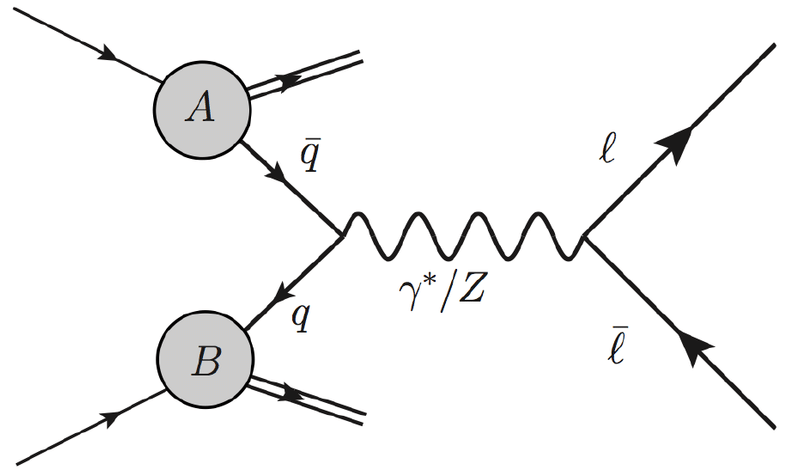
\includegraphics[scale=0.5]{DrellYan.png} 
 	\caption{Leading order Fynnman diagram for Drell-Yan process}
\label{fig:feyn} 
 \end{figure}
\newpage

\section{Underlying events}

Production of Z boson at the LHC can be identified from its decay products, which is the muon anti-muon pair in this case. These muons are highly energetic and isolated as discussed later.  However in a given proton-proton collision muons from Z decay are unavoidably embedded amongst other particles which are produced in the interaction among remaining partons, collectively termed as the underlying event (UE). Thus a good understanding of the properties UE using Monte Carlo (MC) event generators is important. Table~\ref{tab:ue} presents the kinematic properties on average for some of the dominantly produced particles. It is evident that final state of proton-proton collision consists of large number of charged pions ($\pi^\pm$) and photons ($\gamma$) in addition to the particles from the hard scatter. The photons mainly originate from the decay of neutral pions ($\pi^0$). It is evident that the particles from UE are only moderately energetic, therefore the hard scatter part of the event can be isolated by selecting muons with high transverse momenta and not surrounded by other energetic particles. 

\begin{table}
\caption{Characteristics of particles in underlying event in Drell-Yan process}
\begin{center}
	\begin{tabular}{|c|c|c|c|c|c|}
		\hline
		Particle & $<N>$ & $<p_T>$ GeV & $<p_Z>$ GeV & $<\eta>$& $<y>$ \\
		\hline
	   $\gamma$ & 195.8 & 0.3489& 8.412& 0.00032& 0.00032\\
				\hline
		$\pi^+$ & 82.61 & 0.679& 9.707& 0.002249 &0.001644\\
		\hline
		$\pi^-$ & 81.92 & 0.678& 9.63& 0.001731 &0.002131\\
	    \hline
		$K_L$ & 9.293 & 1.113& 12.29& -0.0027  &-0.00259\\
		\hline

				
	   $p$ & 6.828 & 1.083& 14.28& -0.00034& -0.0011\\
	   \hline
	   $n$ & 6.571 & 1.093& 14.23& 0.00143& 0.00029\\
	   \hline							
	\end{tabular}
\end{center}
\label{tab:ue}
\end{table}

\subsection{Jets in underlying events }

It is to be noted that the initial state radiations (gluons as well as photons)from the quarks in the Drell-Yan process are considered as part of UE. The radiated gluon  which carry a fraction of the momentum of the parent quark later forms a shower of mostly hadronic particles. There can be multiple gluon emissions. Therefore the Z is produced along with the jets which give a net transverse boost to the Z boson and consequently to the lepton anti-lepton pair in the final state. If the gluon is emitted at large angle wrt the beam direction, the transverse momentum $(p_T)$ of the jet is large and it can then be detected in the experiment. In the current study we have reconstructed jets through anti-kt algorithm with distance parameter $ R_0 = \sqrt{\Delta \eta^2 + \Delta \phi^2} = 0.4$ and  $p_T > 5$ GeV in the pseudorapidity range of the detector i.e. $|\eta|<5.0$.  The corresponding momentum distribution of jets and the Z boson are shown in the Fig.3. It is evident from the distributions that these jets are mainy soft in nature. Hence the transverse momnetum of the Z particle is also peaked at a reasonably low value of about 5 GeV.

\begin{figure}[h]
	\begin{center}
		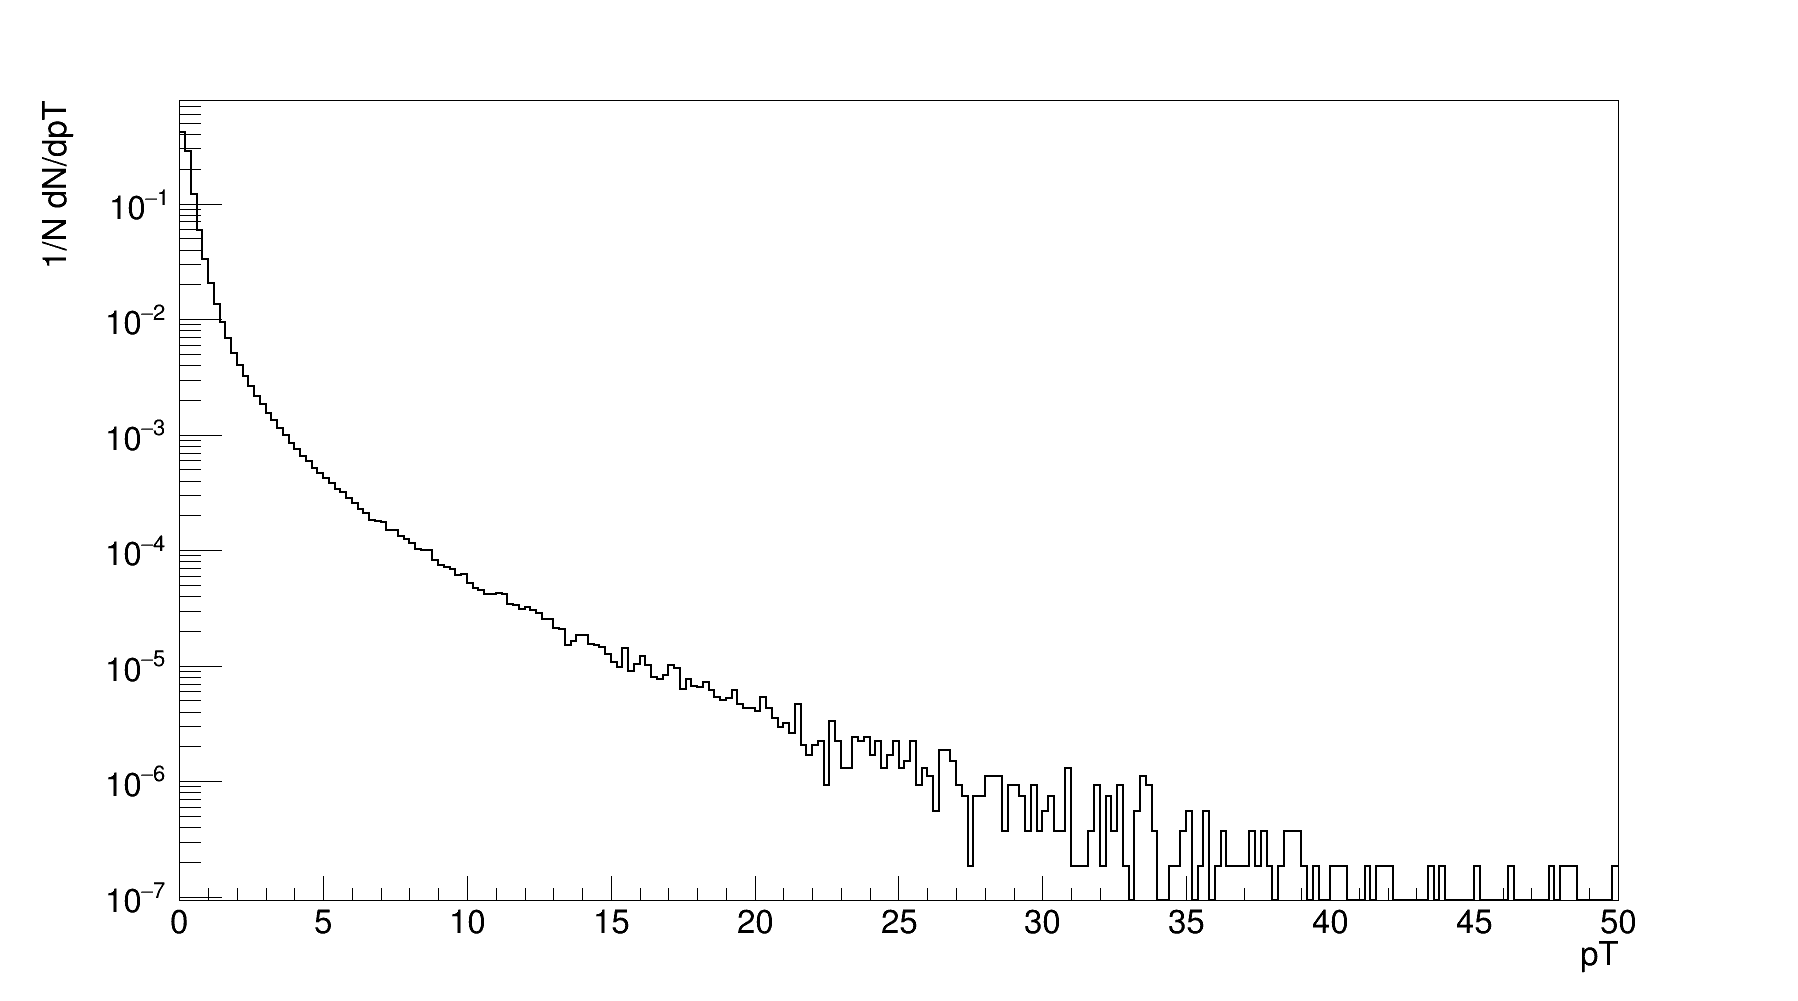
\includegraphics[width=80mm,height=70mm]{jetpt.png} 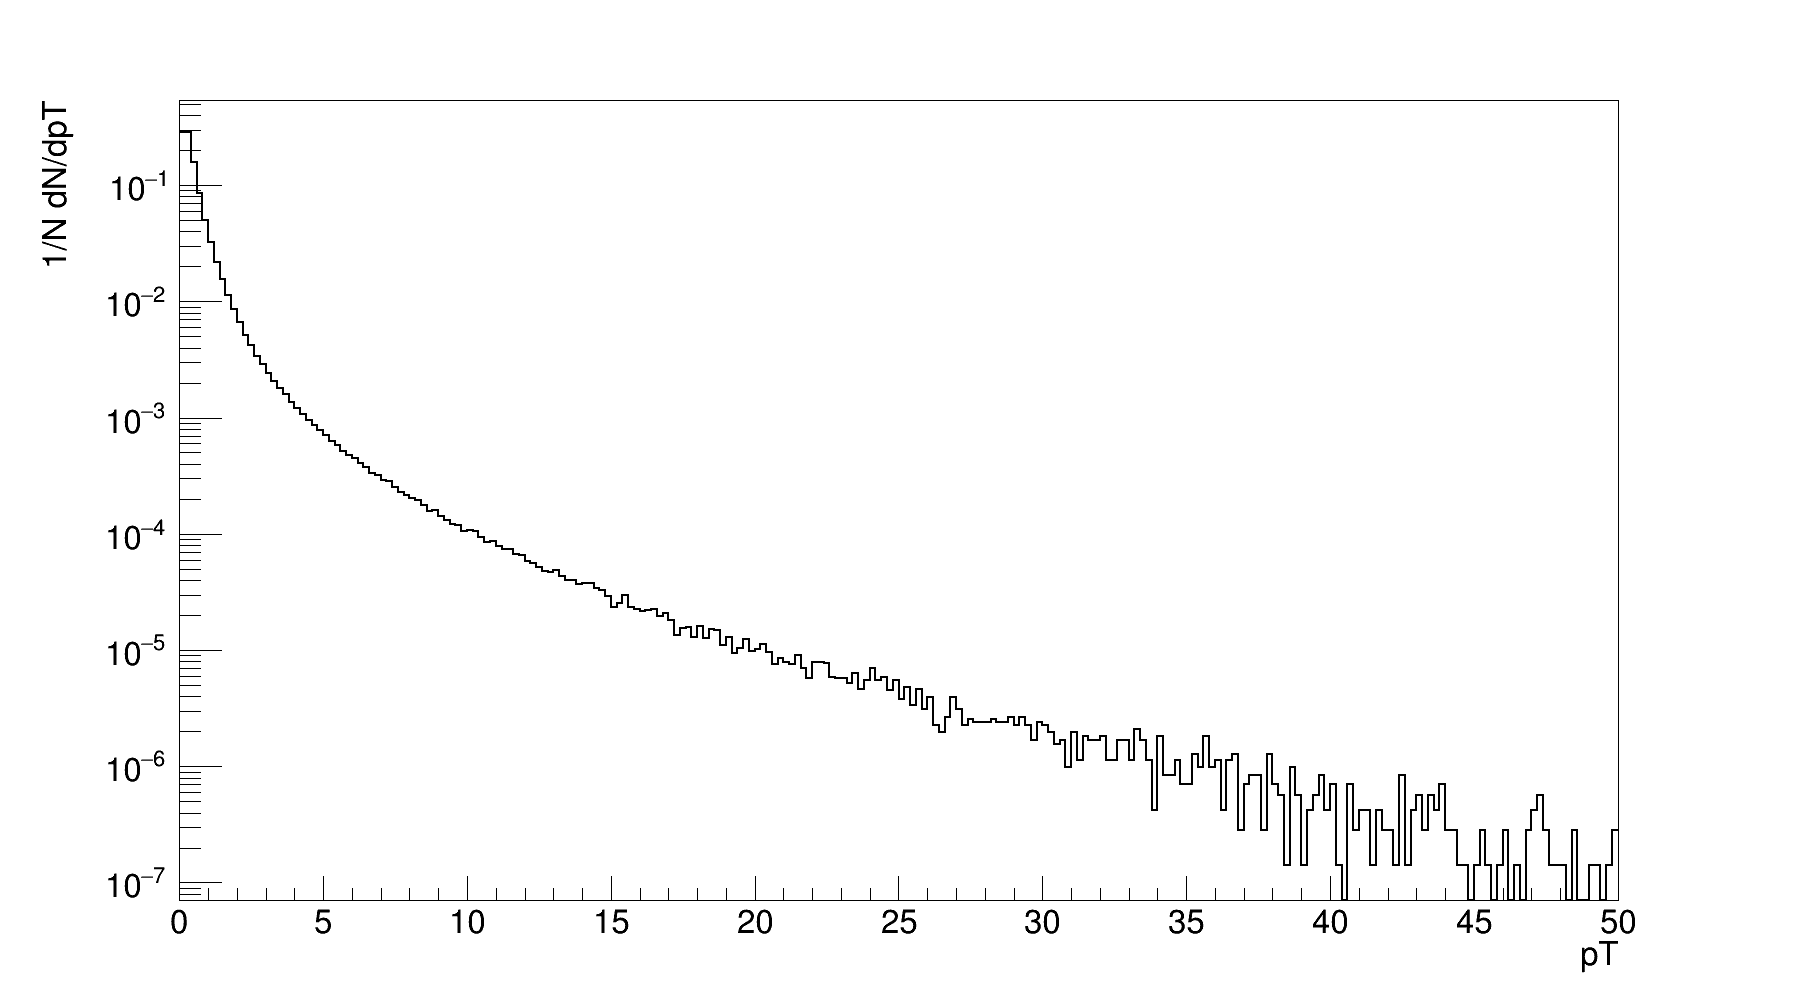
\includegraphics[width=90mm,height=70mm]{zetpt.png} 
		\caption{Transverse momentum distribution of initial state gluon jets in the Drell-Yan process $q\bar{q} \to Z \to \mu^+\mu^-$ (left) and Z particle (right)}.  					
	\end{center}
	\label{fig:zjets}
\end{figure}

Table 3 presents the fraction of number of events with given number of jets which have transverse momentum greater than the threshold values. 

\begin{table}
\begin{center}
\caption{Exclusive jet multiplicities as function of transverse momentum threshiold, normalised to the total number of jets.}
	\begin{tabular}{|c|c|c|c|c|c|}
		\hline
	jet $p_T$ threshold & 1 jet events& 2 jet events& 3 jet events & 4 jet events & 5 jet events \\
		\hline
	10 & 0.27 & 0.17 & 0.082 & 0.039& 0.017\\
	\hline
	20 & 0.177 & 0.046 & 0.01 & 0.002 & 0.0008\\
	\hline
	30 & 0.076 & 0.015 & 0.002 & 0.0006 & 0.0002\\
	\hline
	40 & 0.026 & 0.005 & 0.0005 & 0.0001 & 0\\
	\hline				
	50 & 0.009 & 0.002 & 0.0002 & 0.0001 & 0\\
	\hline
	\end{tabular}
\end{center}
\label{tab:jmult}
\end{table}

\newpage
\section{Signal and background characteristics}

\subsection{Signal}
A reconstructed event of a given final state in the experiment has to satisfy certiain criteria in order to be considered  as signal. 	To identify the decay  $Z \to \mu^+\mu^-$ we require the following conditions to hold true.   
				\begin{enumerate}
					\item The event consists of two oppsitely charged final state muons.
					\item Both of the muons having high transverse momenta $(p_T)$. Fig.~\ref{fig:spt} shows the transverse momentum distribution of the muons in the signal events. 
			
					\begin{figure}[h]
					\centering	
					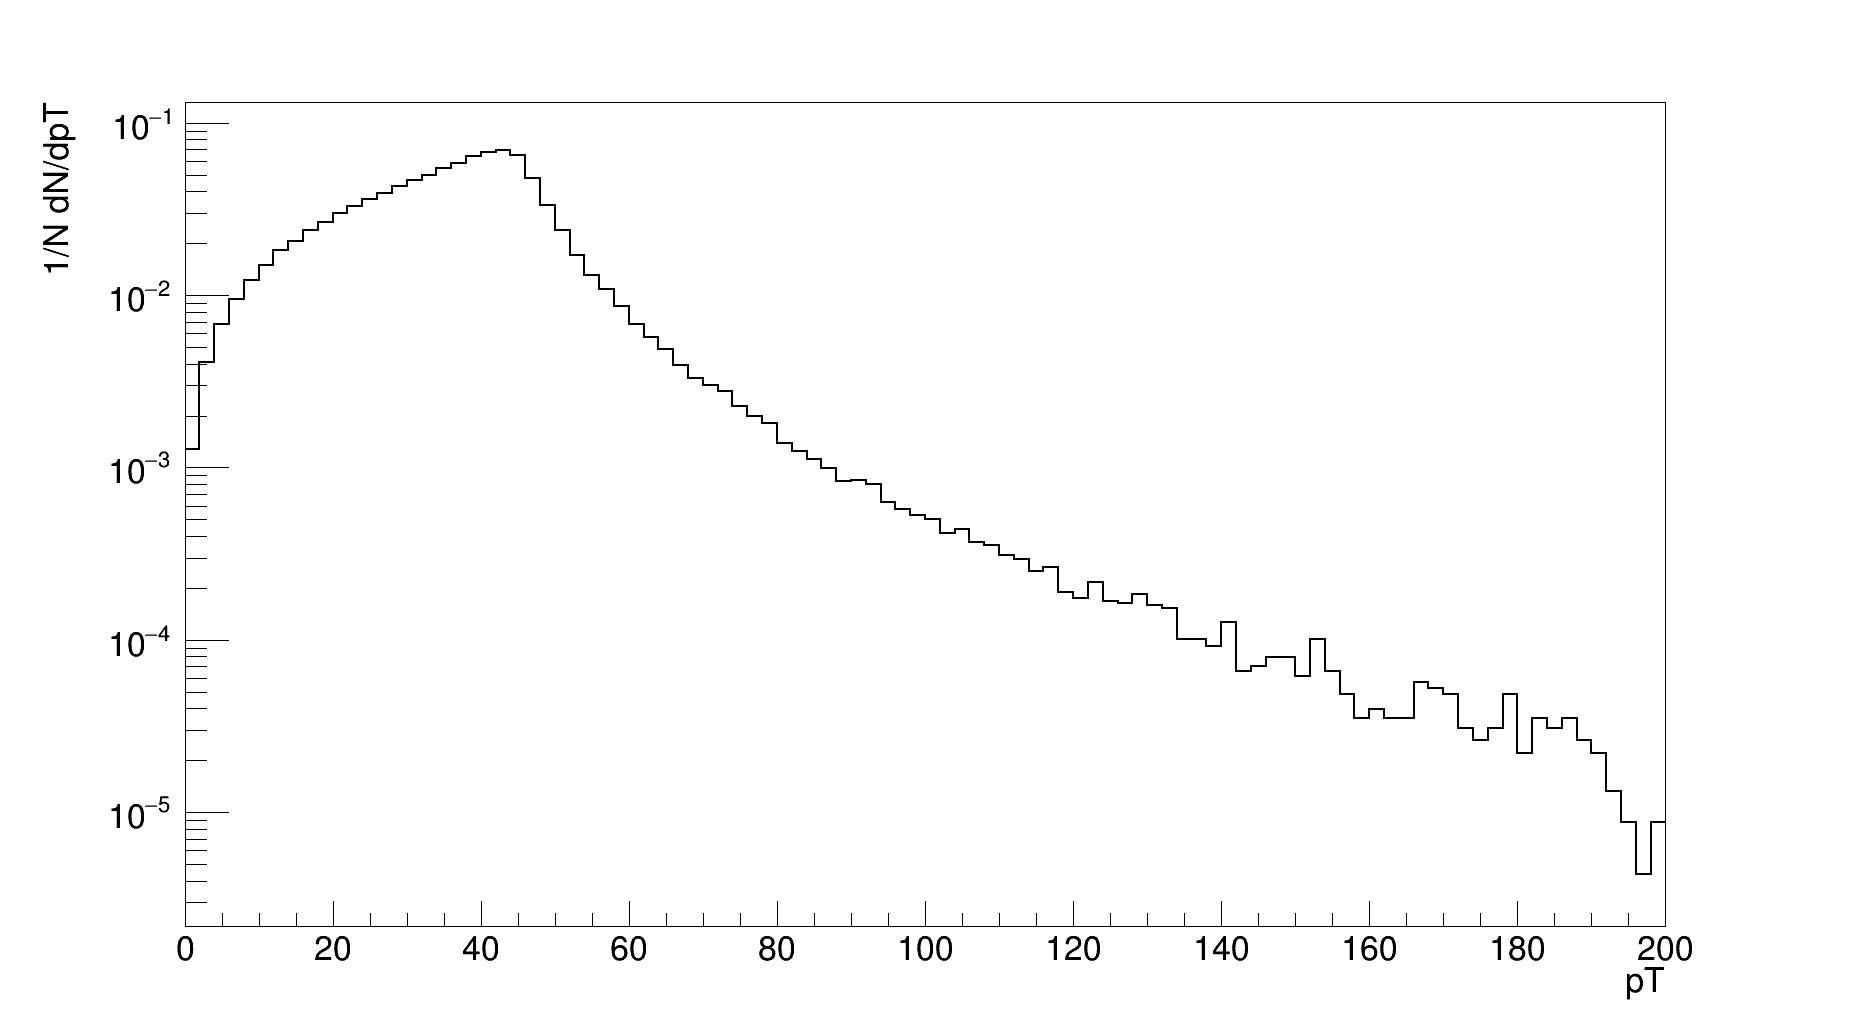
\includegraphics[width=130mm,height=70mm]{signalpt.png} 
					\caption{ Relative isolation variable distribution of the muons in the signal events.}			
					\label{fig:spt}			
					\end{figure}
					
					
					\item Both of the muons being isolated in the cone radius of 0.3 in $(\eta,\phi)$ plane. The cone radius is defined as $\Delta R = \sqrt{\Delta \eta^2 + \Delta \phi^2}$. The relative isolation variable  is defined as $I = \frac{1}{p_T^{\mu}}\sum_{\Delta R< R_0 }^{} p_T^{hadron}$. Distribution of $I$ for the muons in signal events is shown in the Fig.~\ref{fig:mupt}.
					
					\begin{figure}[h]
						\centering	
						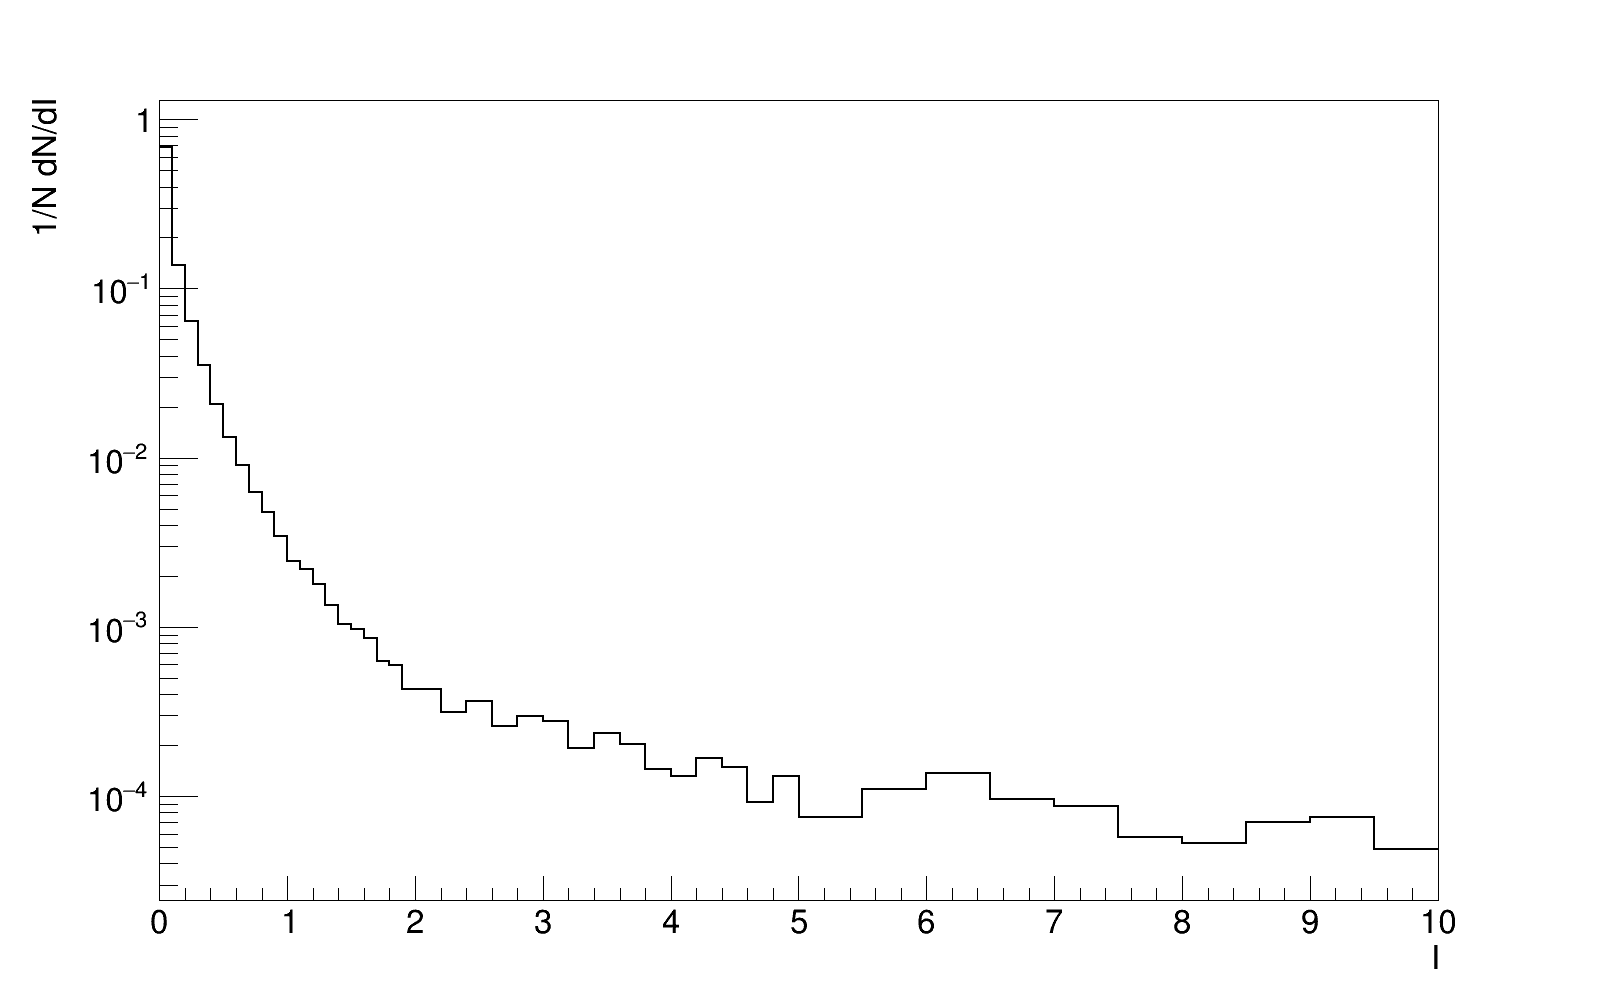
\includegraphics[width=130mm,height=70mm]{is.png} 
						\caption{ Relative isolation variable distribution of the muons in the signal events.}			
                    \label{fig:mupt}			
					\end{figure}
						
					
					\item Both of the muons being in central region of the detector. i.e satisfying $|\eta|<2.5$.	  
				\end{enumerate}
				

\subsection{Background}	
				The final states satisfying signal selection criteria can originate from other physical process. Events containing these final states are termed as background.
			
					    For the decay process $Z \to \mu^+\mu^-$ the possible backgrounds are-
							\begin{enumerate}
								\item QCD induced hadronic interaction processes have total inelastic cross section of around 56 mb at center of mass energy $\sqrt{s} = 13$~TeV compared to the Z decay process with  $\sigma \times BR \approx 0.2nb$, 
								and in a large enough sample these processes can result in final state which mimics signal. These muons however contribute maximally to low $p_T$ region of the spectrum as shown in Fig.6. A minimum momentum threshold is therefore used in order to elimiate these background events.
								
	Muons produced in semi-leptonic decays are accompanied by other particles mainly along the same diretion, and therefore are not "isolated". The relative isolation variable defined as sum of transverse momenta of all final state particles in the cone radius $R_0 = 0.3$ around the final state muon, normalized to the $p_T$ of the muon$(I = \frac{1}{p_T^{\mu}}\sum_{\Delta R< R_0 }^{} p_T^{hadron})$
	is used to discriminate singal against such backgrounds. Muons populating higher values of the distribution are more likely to be from background events.  
								
							
								\begin{figure}[h]
									\begin{center}
										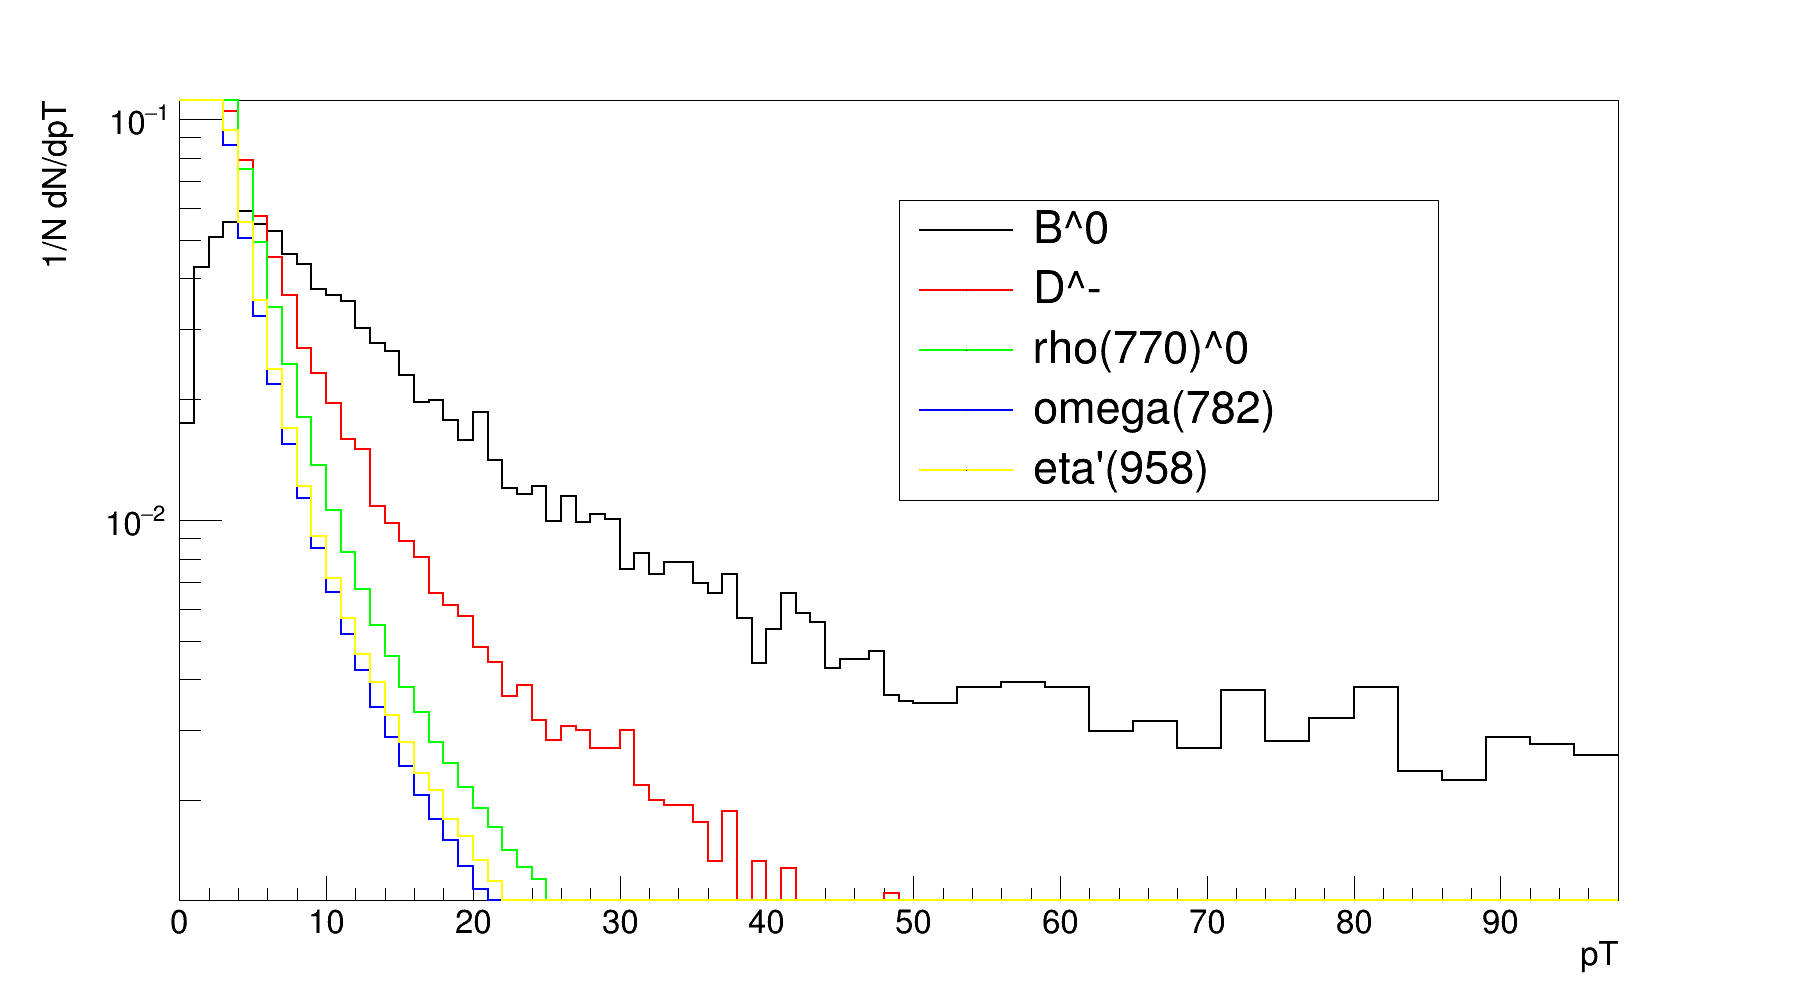
\includegraphics[scale=0.2]{T.png} 
										\caption{$p_T$ Distribution of muons from QCD hadronic decays }	
										\label{hard_pT}				\end{center}
								\end{figure}
																\begin{figure}[h]
																	\begin{center}
																		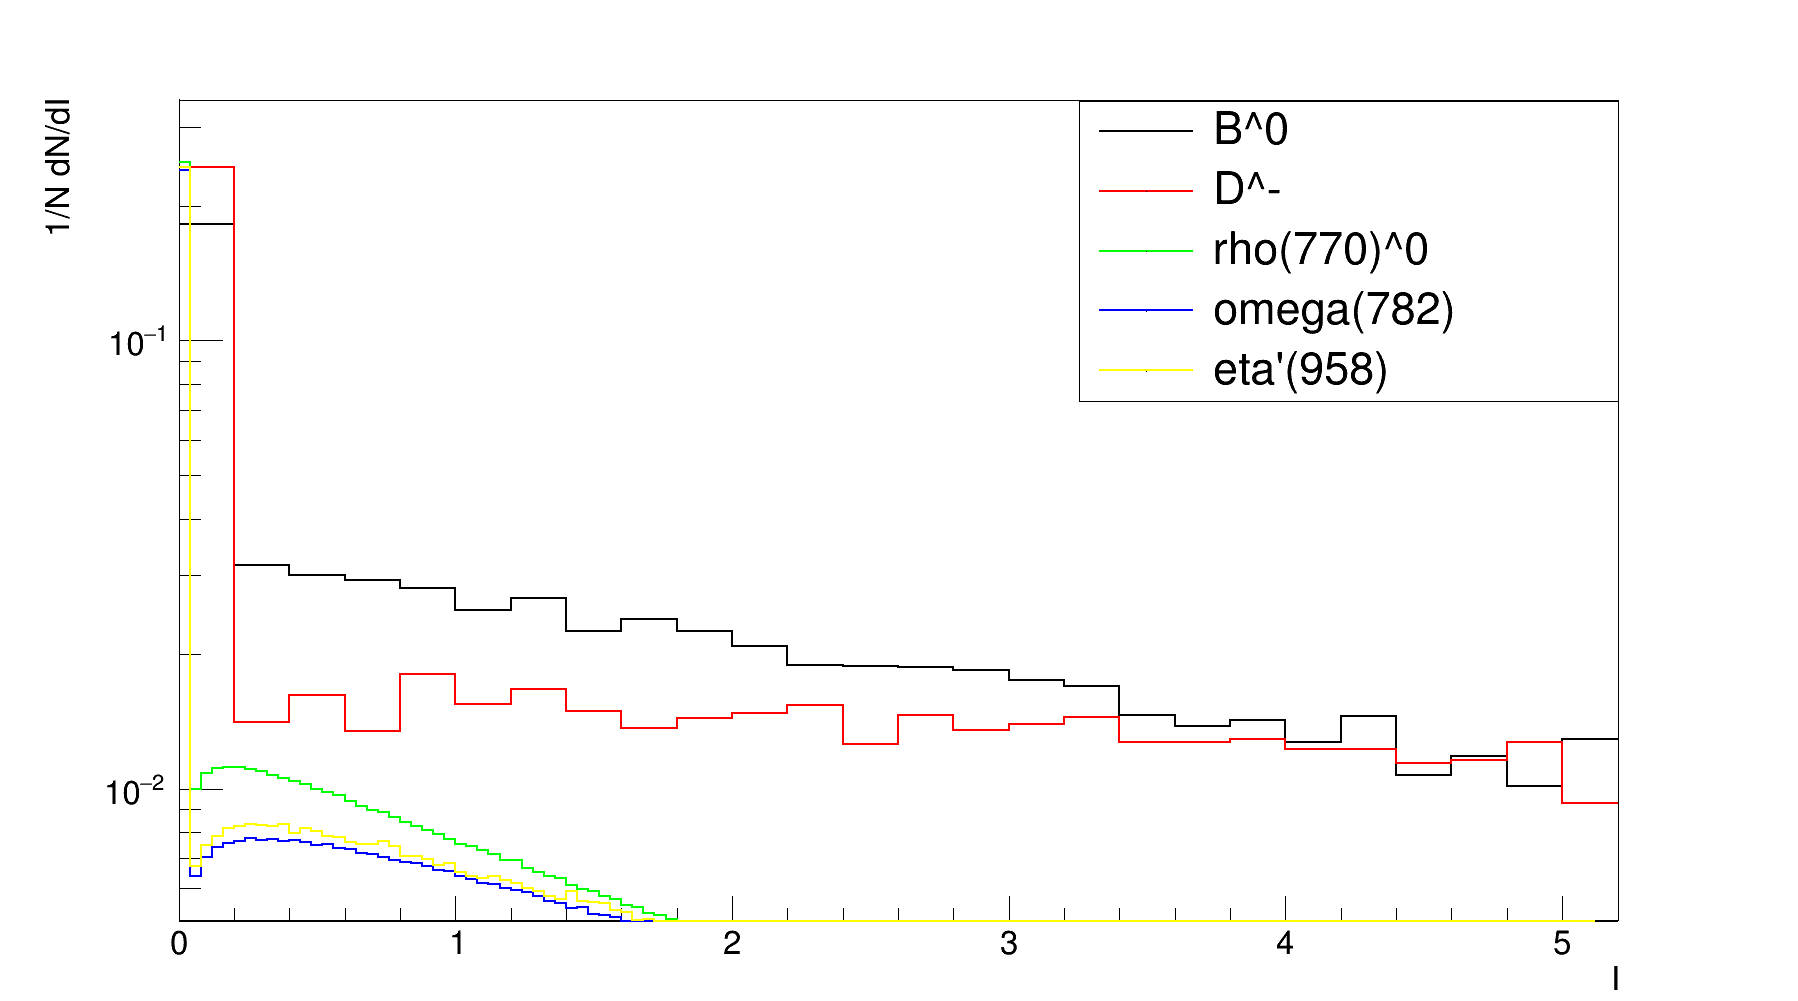
\includegraphics[scale=0.2]{II.png} 
																		\caption{Relative isolation distribution of muons from QCD hadronic decays }	
																		\label{hard_isolation}
																	\end{center}							
																\end{figure}
																						 						
							
								\item W+ jets events with W decaying through muon channel and the highest $pT$ jet faking as muon can also pose as background. A low $p_T$ threshold of about 20 GeV can reduce this background to about $10^{-5}$ level, but the production rate of W boson is high.
								
								\item $t \bar{t}$+jets have large rates, and the cascade decay $t \to W^+q$ , $W^+ \to \mu^+ \nu_{\mu}$  can be source of two energetic isolated muons in the final state with resonably large invariant mass.
								
								\item The process $Z \to \tau^+\tau^- \to \mu^+\mu^- + X$ can also pose as background. The invariant mass of the final state muon however peaks at a lower value as compared $Z \to \mu^+\mu^-$, due to missing energy.     
								 
								\item Diboson production such as WW,WZ,ZZ and their corresponding leptonic decay can also pose as background but with very low rate.
								   
							\end{enumerate}
							In this study only QCD multijet background has been considered in order to optimise signal selection criteria.		    
									    
 \newpage
\section{Event selection cuts}


Signal and background are simulated separately with large number of events. The events selection cuts for transverse momenta and relative isolation are decided by comparing signal distributions to the corresponding total background distributions (both normalized to total number of events), and analyzing signal and background acceptances by changing one of the two bounds of the parameter's cut value separately for each parameter. The selection criteria is deliberately kept lenient in order to have good statistics. Pseudo-rapidity $\eta$ cut is decided to cover the central region of the detector i.e $|\eta|< 2.5$.  
  
\subsection{Transverse momenta}   
The $p_T$ distribution of the signal and QCD background is shown in Fig.8. The background dominates in low(0-20 GeV) $p_T$ region of the distribution due to relatively light mass of the mother particles. The $p_T$ distribution of signal peaks around $\frac{M_Z}{2} = $45 GeV and then dies off, since quite often the Z boson is boosted in the transverse direction as well when accopanied by jets. Therefore a low $p_T$ threshold can be for seperating signal from background i.e. if we select events with both muons satisfying $p_T > p_T^{threshold}$ then the selected sample will have significantly smaller contribution from the background compared to signal. 

\begin{figure}[h]
	\begin{center}
		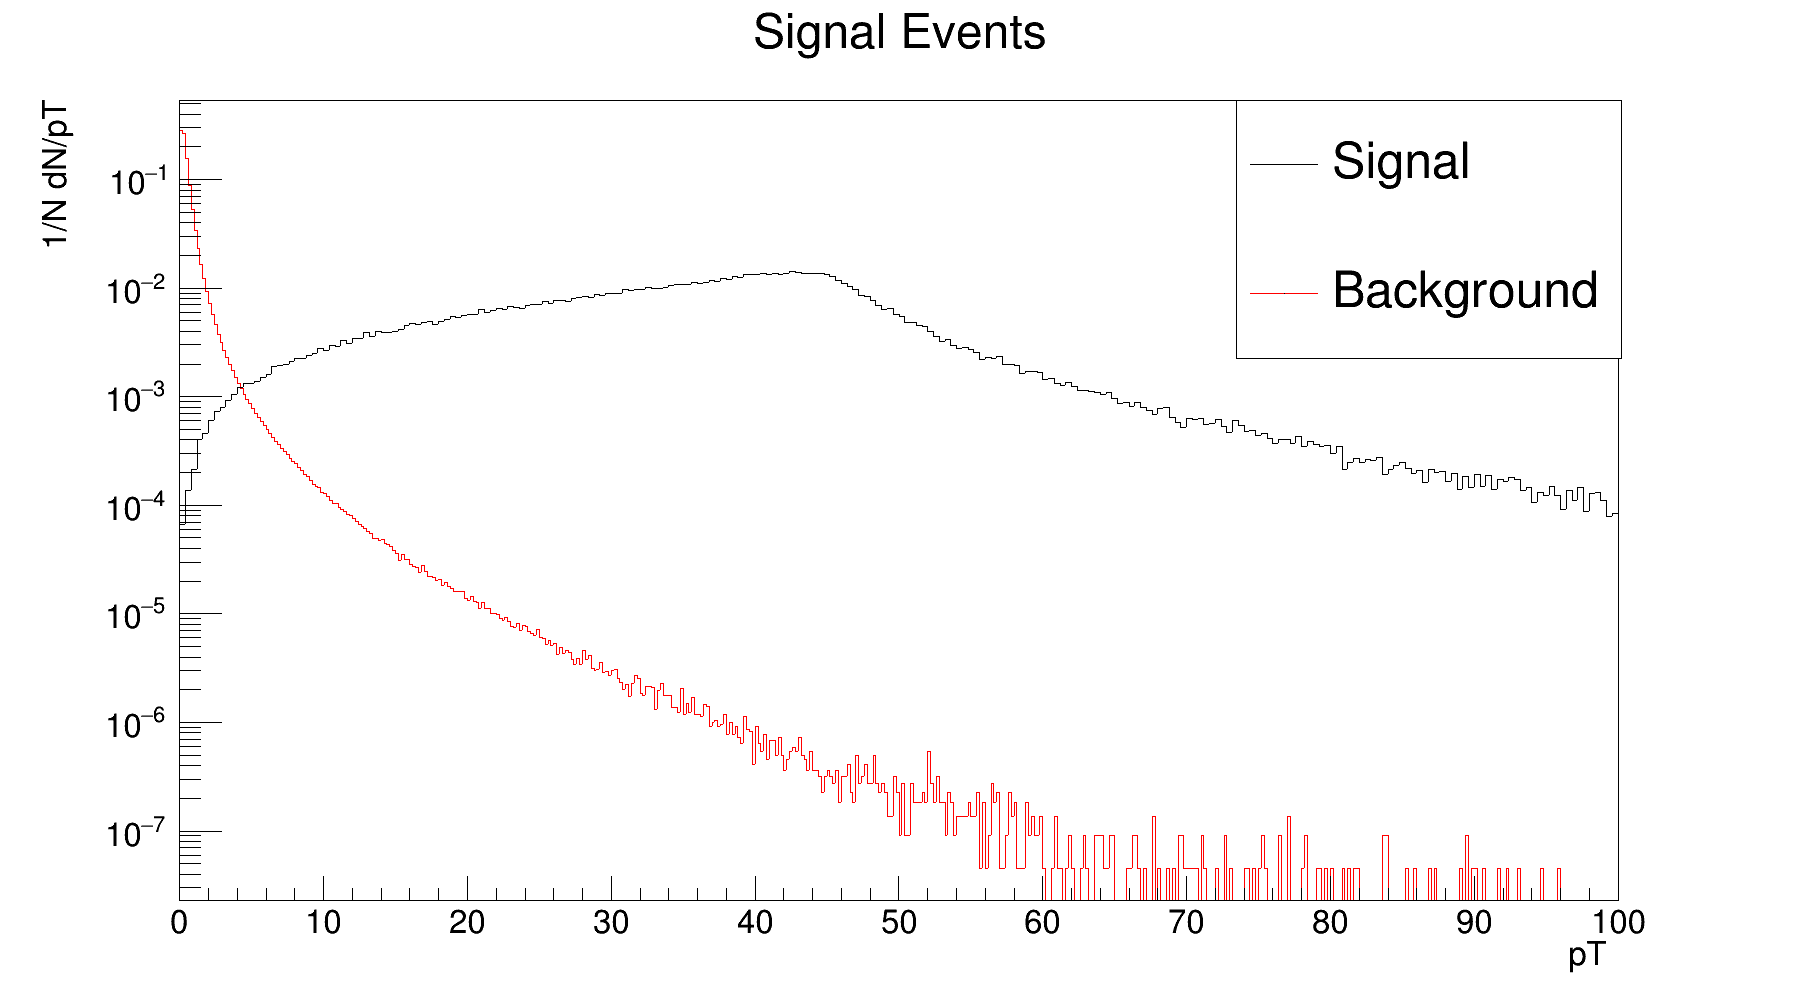
\includegraphics[scale=0.17]{pT.png} 
		\caption{Transverse momentum distribution for signal and background events}		
	\end{center}
	\centering	
\end{figure}						    
\begin{figure}[h]
	\begin{center}
		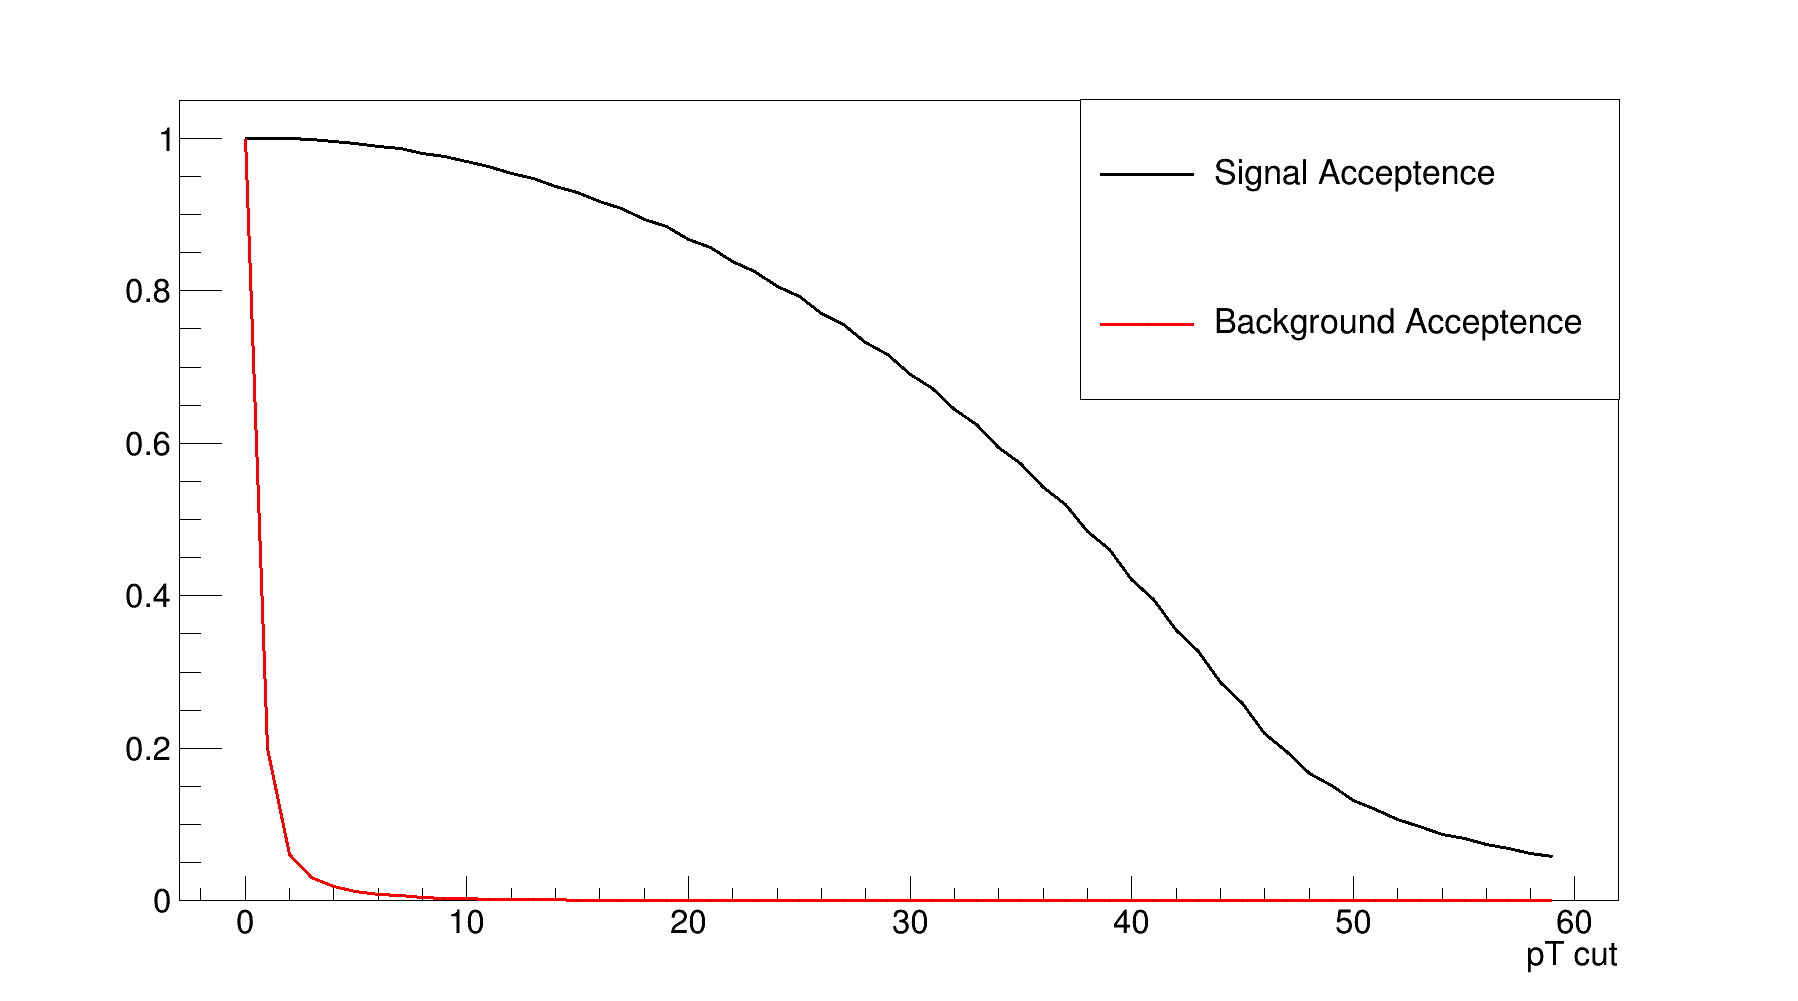
\includegraphics[scale=0.17]{acceptence.png} 	
		\caption{Signal and background acceptance for various $p_T$ treshold.}		
	\end{center}
	\centering	
\end{figure}						    

Signal and background acceptance for different values of  $p_T^{threshold}$ cut are shown in Fig.9 . Most of the background is eliminated with a cut of 20 GeV for which signal acceptance is 86$\%$ and background acceptance is about 0.002$\%$ . Therefore when normalised to corresponding cross section values the bakgound in selected sample will be reduced by to orders of magnitude. 


\subsection{Isolation}

In signal events muons are the only final state particles in a given direction generally, except for the particles resulting from underlying event activity. Thus the relative isolation variable (I) is expected to have a distribution which peaks heavily around I=0 and then rapidly falls off. On the other hand QCD muons produced through semi-leptonic decays are accompanied by a shower of hadrons called QCD Jets in addition to the particles from UE activity. These muons are not isolated and the I distribution is expected to spread farther away from I=0. Thus to select signal like events a high I cut is required .i.e all the events which have $I<I^{threshold }$ should be selected.        

\begin{figure}[h]
	\begin{center}
		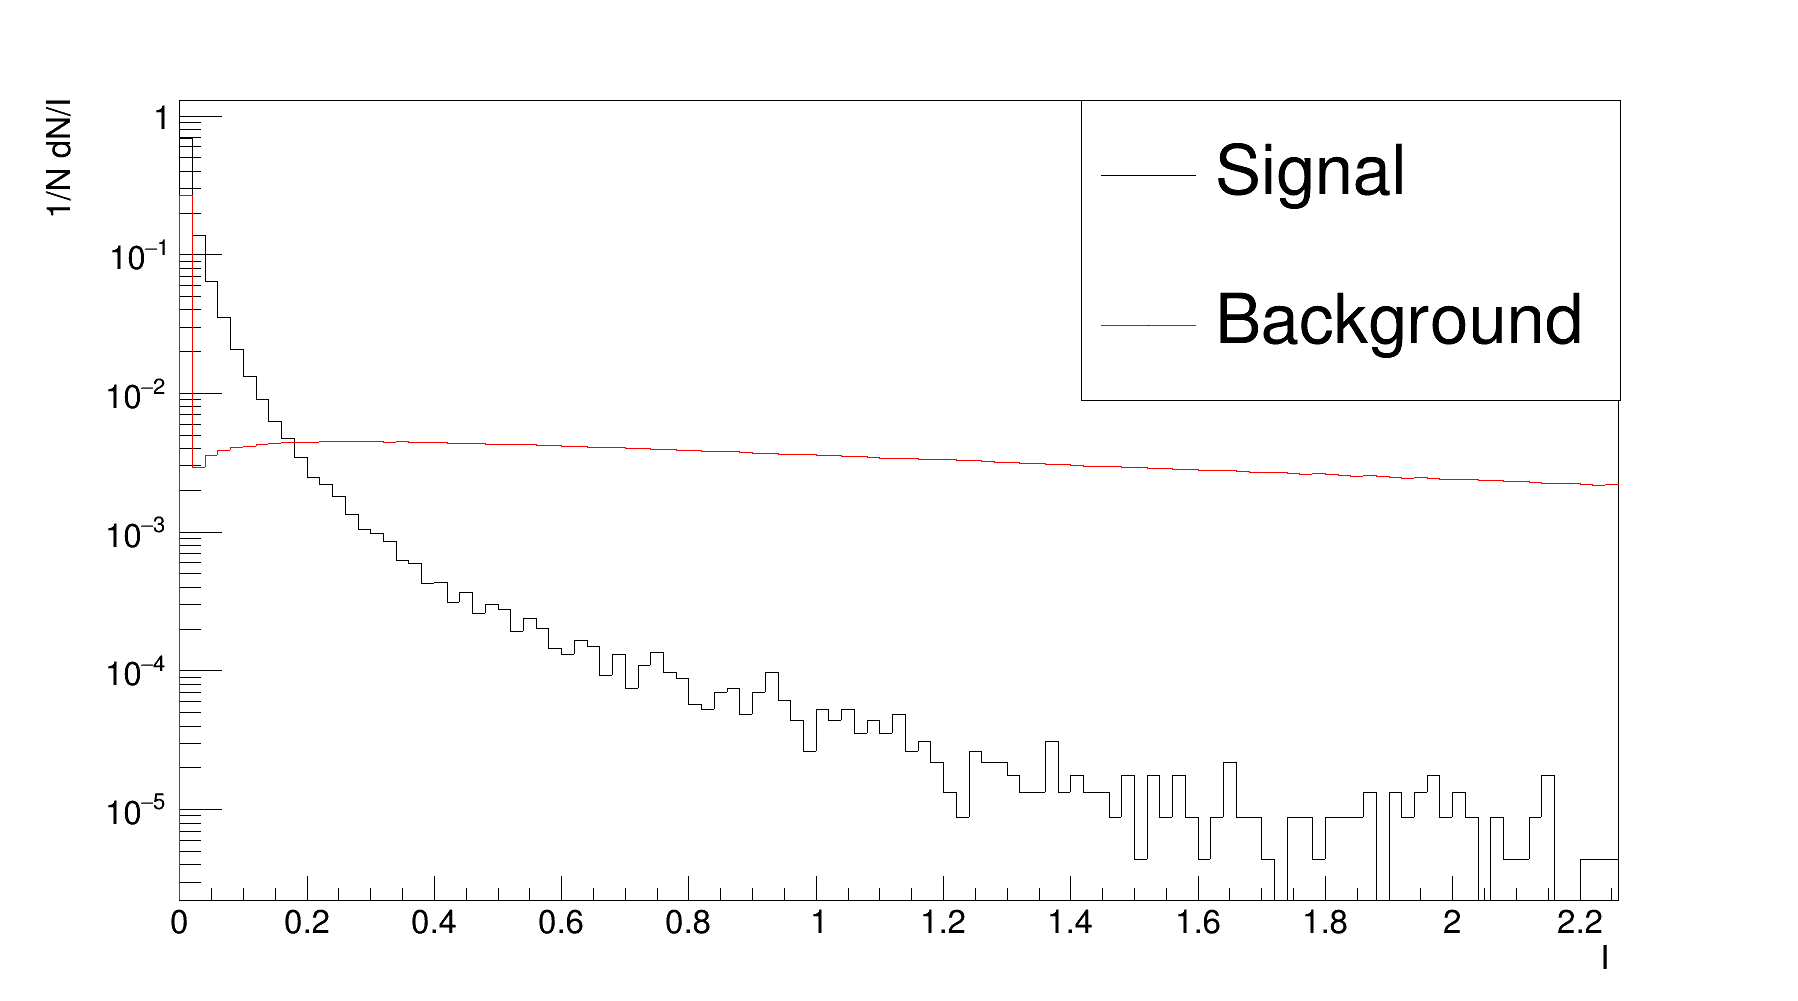
\includegraphics[scale=0.2]{Isvsbg.png} 
		\caption{Relative isolation variable distribution for signal and background events} 		
	\end{center}
	\centering	
\end{figure}
			
Signal and background acceptances for different values of isolation cuts are shown in Fig.11. Maximum signal to background acceptance is achieved for a cut value of 0.11 for which signal and background acceptances are 94$\%$ and 1.5$\%$ respectively.	 	

\begin{figure}[h]
	\begin{center}
		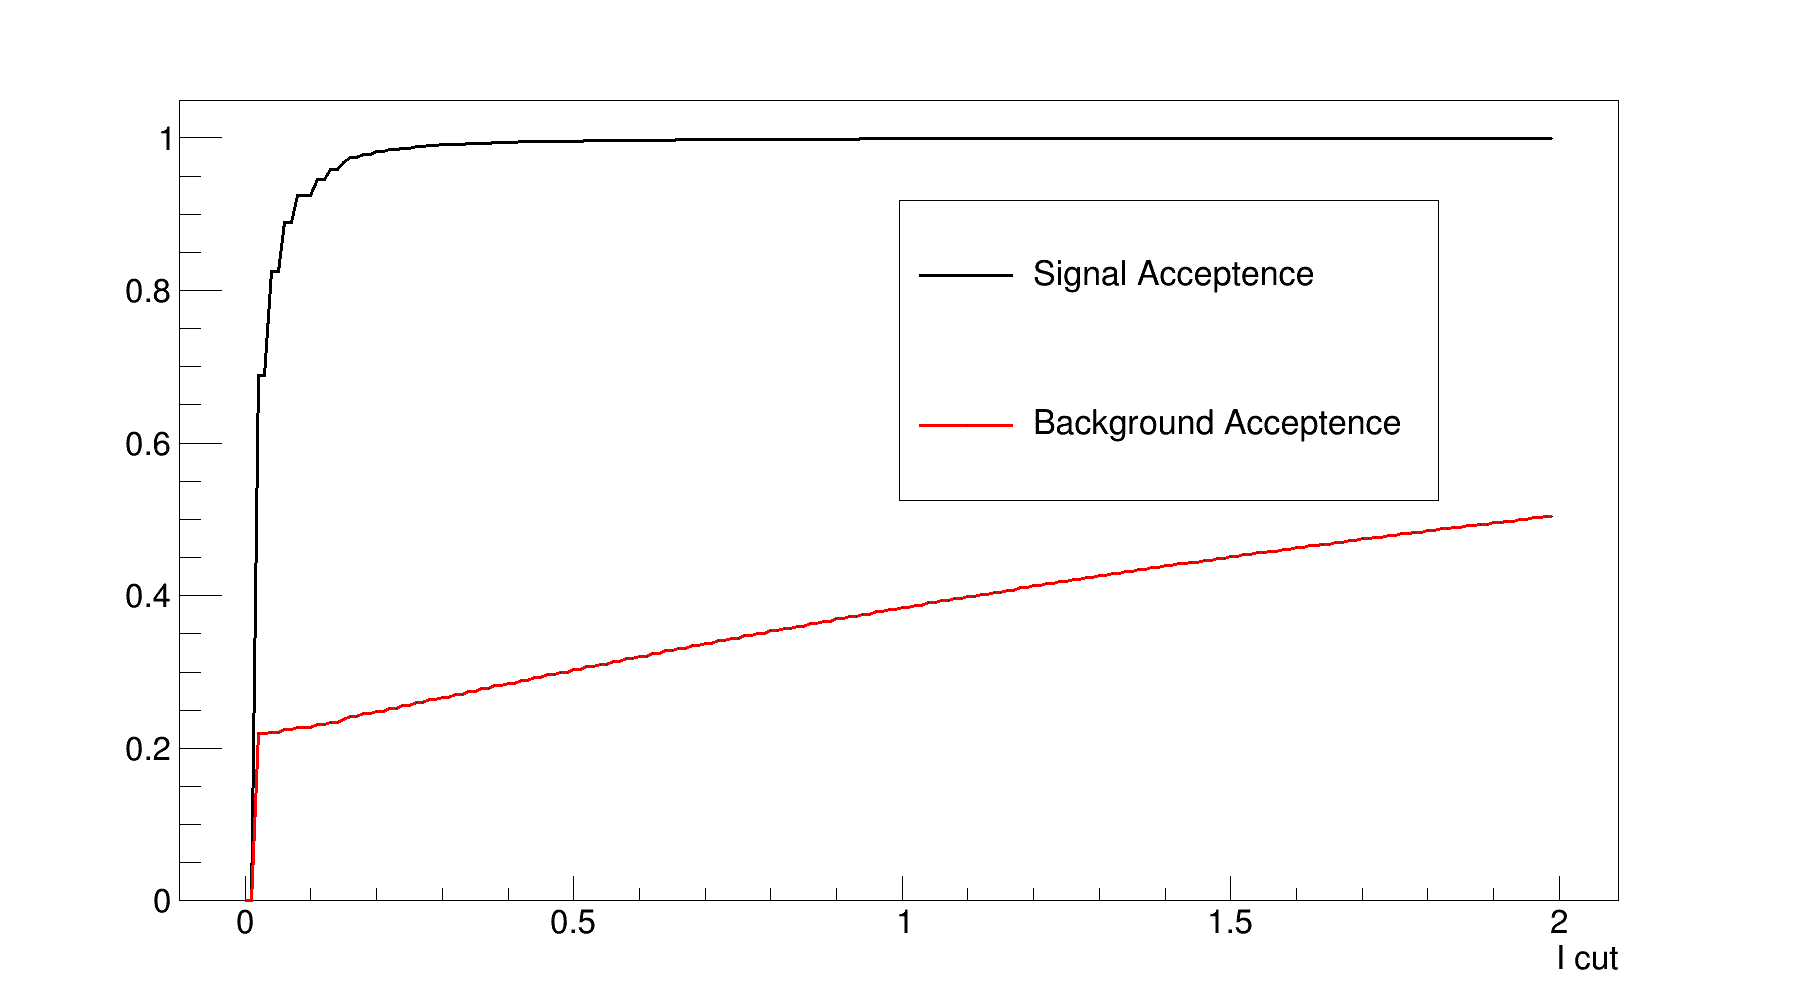
\includegraphics[scale=0.2]{Iacc.png} 
		\caption{Relative isolation variable distribution for signal and background events} 		
	\end{center}
	\centering	
\end{figure}
		

\newpage			
\subsection{Pseudorapidity}  

Muons from QCD multijet events are boosted in forward-backward region therefore their pseudorapidity distribution tend to be spread out to higher values whereas that of muons from $Z \to \mu^+ \mu^-$ are populated in central region, therefore a low $|\eta|$ cut is desired such that events which contain muons with high $|\	eta| $ are rejected. Threshold for $|\eta|$ is chosen to be 2.5 since this defined the central region of the detector.    

\begin{figure}[h]
	\begin{center}
		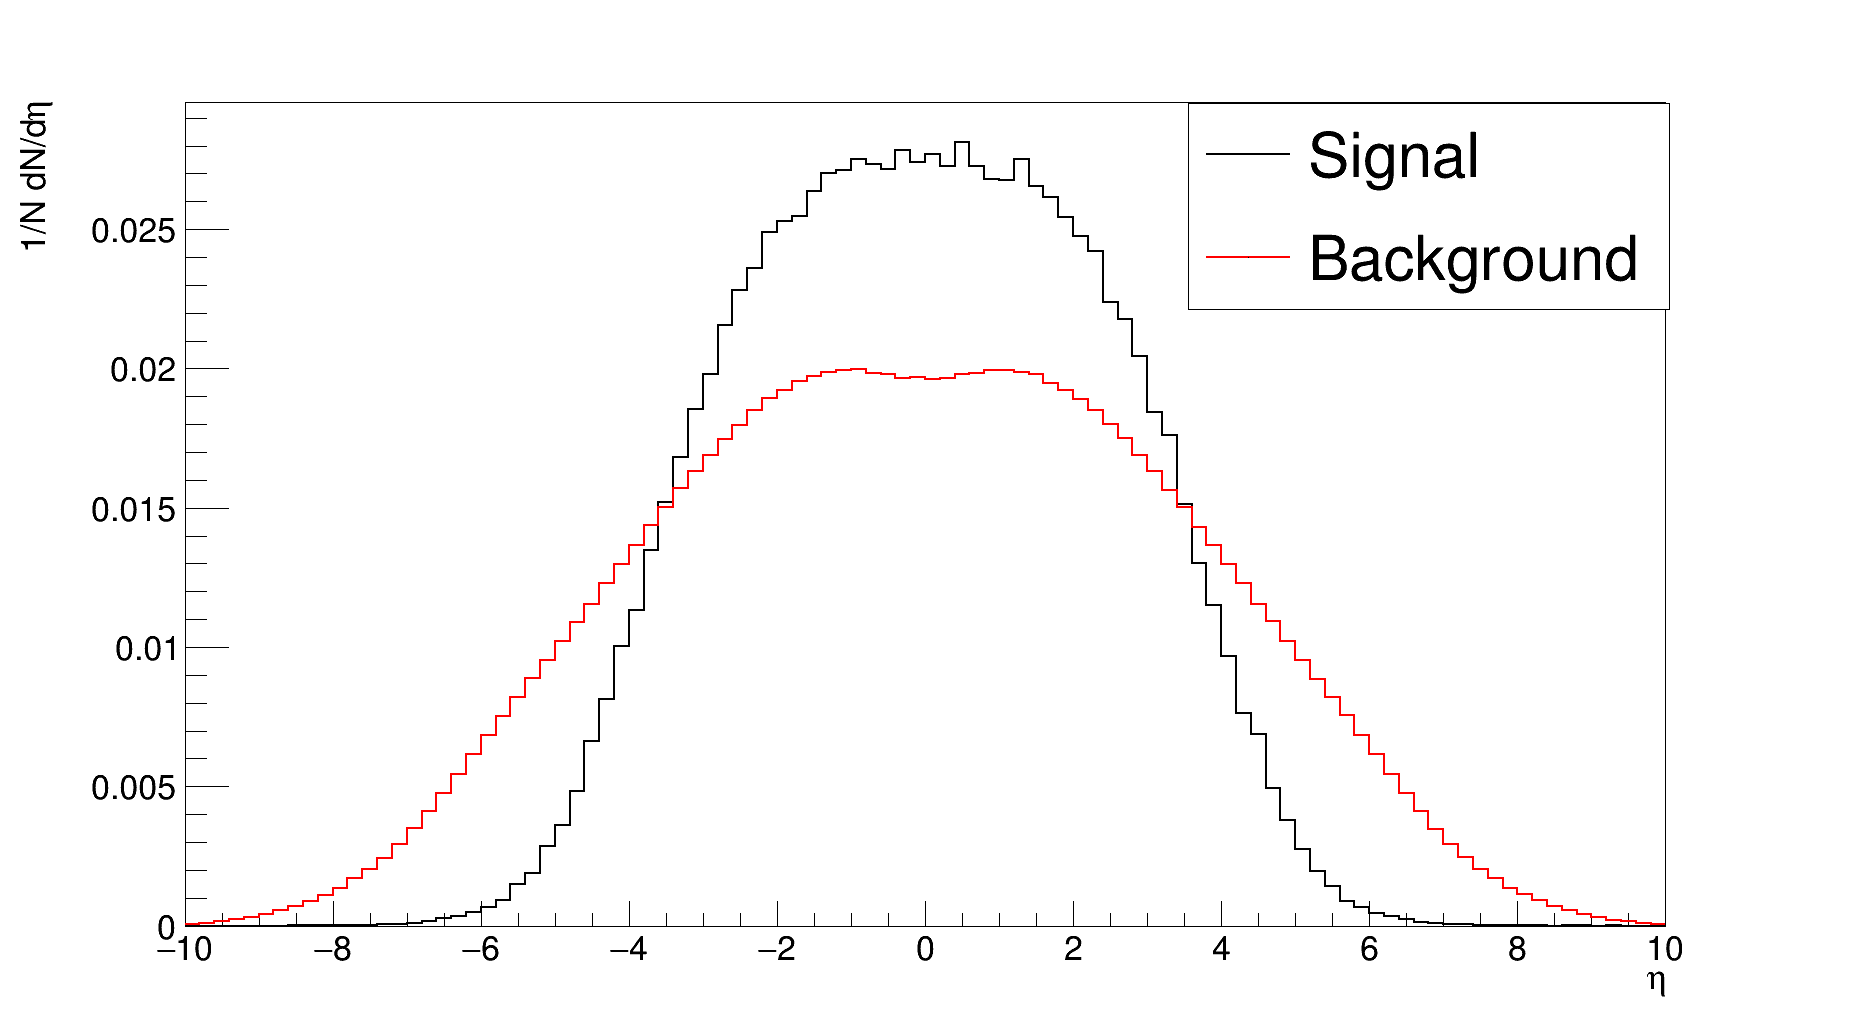
\includegraphics[scale=0.2]{etasvsbkg.png} 
		\caption{Pseudorapidity distribution for signal and background events}		
	\end{center}
	\centering	
\end{figure}						    



\section{Results}

A total of $4 \times 10^6$ highly inelastic hadronic interaction (HardQCD) events are generated and only the event having 2 oppositely charged muons passing all the selection criteria  defined above are selected. The events which do not pass any of the 4 selection criteria are rejected through and OR condition the results are summerized in the table below. 

\begin{center}
	\begin{tabular}{|c|c|c|}
		\hline
		Selection & Single muon events & Events with two oppositely charged muons\\
		\hline
		Total & 372269 & 95948\\
		\hline
	     $I \le 0.11$ & 63261 & 5061\\
		\hline  
		$I \le 0.11$ and $p_T \ge 20$ GeV & 15 & $<1$\\
		\hline
		$I \le 0.11$ and $p_T \ge 20$ GeV and $|\eta| \le 2.5$ & 11 & $<1$\\
		\hline
	\end{tabular}
\end{center}

	With the simulation results it is concluded that fraction of muons from QCD multijet process which can pass all of the three $(p_T,I,\eta)$ selection threshold is about $\frac{11}{372269}$ = $2.95 \times 10^{-5}$ and the fraction of di-muon events which can pass all the selection criteria is $\frac{95948}{4000000} \times \left(2.95 \times 10^{-5} \right)^2 \approx 2.087 \times 10^{-11} $. Therefore the total QCD background level with these selection thresholds is $ 2.087 \times 10^{-11} \times 56.79$ mb = $ 1.1852$ pb. Compare this to total signal level i.e. 0.86 $\times$ 0.94 $\times$ $\sigma(q\bar{q} \to Z) \times BR(Z \to \mu^+\mu^-) = 176$ pb. We get the total signal to background ratio of about 119.64.     		

	

\section{Conclusion}

Events with two oppsitely charged muons with $p_T>20 $ GeV, $|\eta|<2.5$, and $I<0.11$ are selected. Events not satisfying any of the above criteria are rejected through an OR condition, the corresponding signal to background ratio with these selection threshold is found to be 119.64. The invariant mass distribution of the events passing all the above selection criteria is shown in Fig.13 and is observed to have a resonance peak around 91.2 GeV.
A Breit-Wigner fit to the invariant-mass distribution is done with mass(m) and decay widht($\Gamma$) chosen to be parameters for the estimation. The Breight-Wigner fit function is defined as 

	$$BW(x;m,\Gamma,k) = \frac{k}{(x^2 - m^2)^2 + m^2 \Gamma^2}$$	 

where k is normalizing constant.
 
The invariant di-muon mass and decay width obtained from fitting Breit-Wigner to the di-muon mass distribution are 91.1818 GeV and 2.54 GeV respectively. Which are in good agreement with the input values of these parameters.	

\begin{figure}[h]
	\begin{center}
		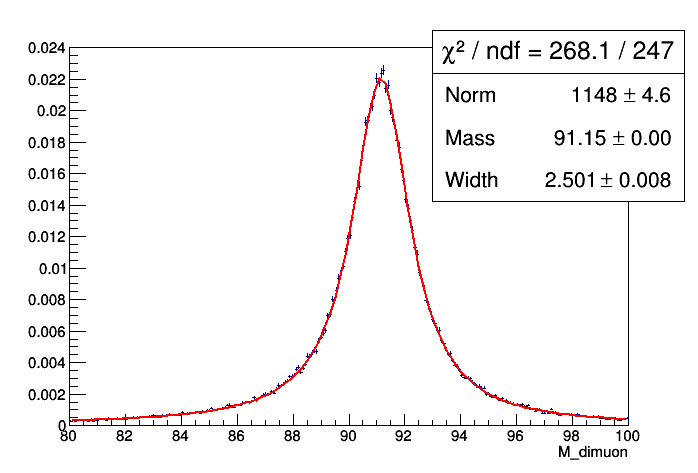
\includegraphics[scale=0.5]{m.png} 
		\caption{Invariant mass distribution of the di-muon passing the selection cuts} 					
	\end{center}
	\centering	
\end{figure}

\section{Ackowledgement}
	I would like to thank my project supervisor Prof. Kajari Majumdar, for providing meaningfull insights to the experimental as well as theoretical aspects of the high energy experiments and guiding me throughout the project. I would also extend my gratitude to Mintu Kumar(DHEP), Uttiya Sarkar(DHEP) for their help regarding various technical and non-technical issues.  
	
\section{Referrences}

  [1]Arno R. Bohm and N. L. Harshman
"\href{https://arxiv.org/pdf/hep-ph/0001206.pdf}{https://arxiv.org/pdf/hep-ph/0001206.pdf}" \\


[2] The LHCb collaboration "\href{https://arxiv.org/pdf/1607.06495.pdf}{Measurement of the forward Z boson production cross-section in pp collisions at $\sqrt{s} = 13$TeV}", 2016.


[3] Lashkar Mohammad Kashif "\href{http://lppc.physics.harvard.edu/files/lppc/files/kashif-2.pdf} {Measurement of the Z boson cross-section in the
	dimuon channel in ppcollisions at $\sqrt{s}= 7 $TeV}"

[4] The CMS Collaboration "\href{https://arxiv.org/pdf/1504.03511.pdf}{Measurement of the Z boson differential cross section in
	transverse momentum and rapidity in proton-proton
	collisions at 8 TeV}" , 2015

[5] Matthias Schott "\href{https://cds.cern.ch/record/2069156/files/Schott_Matthias.pdf}{Study of the Z Boson Production at the ATLAS Experiment with First Data}",2007




	
%	For two body decay of type $0 \to 1+2$ the energies and the masses of the decay products can be written as
	
%	\begin{eqnarray}
%		E_1 &=& \frac{M^2+m^2_1-m^2_2}{2M}\\
%		p_1 &=& \frac{\sqrt{(M^2+-m^2_1-m^2_2)^2-4M^2m^2_1}}{2M} \\
	%	p_2 &=& \frac{\sqrt{(M^2+-m^2_2-m^2_1)^2-4M^2m^2_1}}{2M} 			
	%\end{eqnarray}
    
     %For, the $Z \to \mu^+\mu^-$ decay we have $m_{\mu^+} = m_{\mu^-}<<m_Z$. Therefore we can neglect the square of muon mass compared to Z mass and get $$E_1 = E_2 \approx p_2 = p_1 = \frac{M}{2} = 45.5 GeV $$ .
     
     %Therefore if muons are produced by this process only and there is no background, then the histogram of their total energy will peak at 45.5GeV.
		
 

% \section{ Information so far}
 
 %\textbf{Proposition:} W and Z bosons together are known as "intermediate vector bosons", these elementary particles are the mediators of the weak interaction.\\
%\textbf{Explanation:} First of all a \textbf{boson} is a fundamental particle following Bose-Einstein statistics(Unlimited number of them can "condense" into the same energy state, as opposed to fermions which occupy one state per particle, this distinction between boson and fermion become significant when the interparticle distance is comparable to the De-Broglie wavelength, so that their wavefunctions are partially overlap.Bosons can be fundamental particles such as Photon ,Higgs particle and Graviton or they can be combination of even number of fermions e.g. Helium nuclei. the last example is starting point when you try to explain superfluid nature of Helium. You can also read about $\href{https://en.wikipedia.org/wiki/Spin%E2%80%93statistics_theorem}{Spin statistics theorem.}$ ), in standard model there are four vector bosons($\gamma,g,Z,W^\pm)$  with spin 1 ,one scalar boson $(H^0)$ with spin 0 and one hypothetical Tensor boson$(G)$  with spin 2.   The three W and Z bosons correspond (roughly) to the three generators of SU(2) in GWS theory. The name "vector boson" is used when we talk about particles which have spin 1 and have 3 eigenstates corresponding to spin of -1,0,1. This triplet can be superimposed with other other triplets and one can perform rotations in the spin space. The weak althought affects all fermions , it is short ranged owing to the large masses of W and Z. The weak processes involving W are called "charged current" and that involving Z bosons are calles nautral current interactions. Weak interaction violates parity conservation but was thought to preserve CP symmetry, which was also observed to be violated first by studying decay of Kaon.



\pagebreak
(1)https://www.sciencedirect.com/science/article/pii/0370269383911772
  
(2)http://home.thep.lu.se/Pythia/
 
(3)https://root.cern.ch/ 
 
 
 (5)https://home.cern/about/experiments/cms
 
(6)https://ac.els-cdn.com/S0168900296011060/1-s2.0-S0168900296011060-main.pdf?_tid=0121ba5b-fb98-4e8a-8048-514cfbbd45bfacdnat=1528494088_561397cced66498a448552dff73e5a24 
 
 
\end{document} 


